\documentclass[a4paper,12pt]{article} 
\usepackage{graphicx}
\usepackage{amsmath, amssymb}
\usepackage{hyperref}
\usepackage{geometry}
\geometry{left=1in, right=1in, top=1in, bottom=1in}
\usepackage{caption}
\usepackage{subcaption}
\usepackage{booktabs}
\usepackage{enumitem}
\usepackage{titlesec}
\titleformat{\section}{\large\bfseries}{}{0em}{}
\usepackage{float}  % Add this to the preamble
\usepackage{placeins} % Add this to handle float barriers

\title{\textbf{Margin Calculation and Risk Analysis for Financial Derivatives}}
\author{Vishal Shisodia}
\date{March 6, 2025}

\begin{document}

\maketitle


Financial markets require robust margining systems to ensure that participants maintain sufficient collateral to cover potential losses. This project tries to develop a Python-based tool to compute margin requirements and assess financial risk exposure in derivative markets. By leveraging historical price data, statistical risk metrics, and machine learning techniques, the tool provides insights into initial margin calculation, variation margin tracking, and Value at Risk (VaR). The study explores the impact of volatility and market conditions on margin requirements and assesses the effectiveness of predictive models in risk management. The results indicate that Parametric VaR is the most significant factor influencing margin requirements, and the Random Forest model achieves high predictive accuracy. This project serves as a bridge between theoretical financial risk models and real-world implementation, facilitating better risk management practices.


\section{Introduction}
Risk management in financial derivatives trading is a critical component of market stability. The margining process ensures that traders deposit sufficient collateral to mitigate counterparty risk. Given the dynamic nature of financial markets, accurately estimating margin requirements is essential to prevent excessive leverage and systemic risks.

The aim of this project is to develop an automated computational tool that calculates margin requirements and assesses financial risk exposure using Python. The project integrates statistical financial models, machine learning techniques, and data visualization to enhance risk assessment capabilities. 

With my experience as a working student at an energy company in the Exchange, Clearing, and Marketing Operations department, I have developed a strong interest in understanding and automating risk assessment procedures. The need for accurate, data-driven risk assessment has motivated this research, which seeks to bridge the gap between theoretical finance concepts and practical implementation. 

The primary objectives of this project include:
\begin{itemize}
    \item Automating the calculation of initial and variation margins for futures contracts.
    \item Implementing statistical risk measures such as Value at Risk (VaR) to quantify market exposure.
    \item Developing a machine learning model to predict future margin requirements based on historical volatility and market trends.
    \item Visualizing key risk metrics to facilitate better decision-making in financial risk management.
\end{itemize}

\section{Methodology}
The methodology consists of five key steps, each contributing to a comprehensive analysis of margin requirements and financial risk:

\begin{enumerate}
    \item \textbf{Data Collection}: Historical market data for natural gas futures is retrieved using the \texttt{yfinance} API to ensure real-time applicability.
    \item \textbf{Data Processing}: Cleaning and feature engineering are performed to calculate key indicators such as daily returns and rolling volatility.
    \item \textbf{Risk Metrics Computation}: Initial margin, variation margin, and Value at Risk (VaR) are calculated to quantify risk exposure.
    \item \textbf{Machine Learning Modeling}: A Random Forest Regressor is trained to predict initial margin requirements based on volatility and VaR metrics.
    \item \textbf{Visualization and Analysis}: The impact of risk factors on margin requirements is analyzed using graphical representations.
\end{enumerate}



\section{Implementation: Scripts and Steps Involved}
This project is structured across multiple Python scripts, each contributing to different phases of the analysis:

\subsection{Fetching Data (\texttt{fetch\_data.py})}
This script retrieves historical price data from Yahoo Finance.
\begin{itemize}
    \item Defines the futures contract ticker (e.g., "NG=F" for Natural Gas Futures).
    \item Fetches historical prices between specified dates (from 2021-01-01 to 2024-01-01).
    \item Saves the data as a CSV file for further processing.
\end{itemize}

\subsection{Data Cleaning and Preprocessing (\texttt{clean\_data.py})}
This script processes raw market data to prepare it for risk analysis.
\begin{itemize}
    \item Loads the CSV file and renames columns for consistency.
    \item Computes daily returns and rolling volatility.
    \item Handles missing values by dropping incomplete rows.
    \item Saves the processed data for further analysis.
\end{itemize}

\subsection{Computing Risk Metrics (\texttt{risk\_analysis.py})}
This script calculates key financial risk metrics.
\begin{itemize}
    \item Computes \textbf{Initial Margin} based on market volatility.
    \item Tracks \textbf{Variation Margin} to measure daily profit/loss dynamics.
    \item Computes \textbf{Value at Risk (VaR)} using historical and parametric methods.
    \item Saves the computed risk metrics to a CSV file.
\end{itemize}

\subsection{Training the Machine Learning Model (\texttt{train\_model.py})}
This script trains a Random Forest model to predict Initial Margin.
\begin{itemize}
    \item Splits data into training and testing sets.
    \item Standardizes features for better model performance.
    \item Trains a Random Forest Regressor with key risk factors.
    \item Evaluates the model using MSE and R-squared score.
\end{itemize}

\subsection{Visualizing Risk Metrics (\texttt{visualize\_results.py})}
This script generates plots for Value at Risk (VaR) and other risk metrics.
\begin{itemize}
    \item Plots historical vs. parametric VaR over time.
    \item Highlights periods of high risk exposure.
    \item Saves the visualizations as high-quality PNG files.
\end{itemize}





\section{Results and Analysis}

\subsection{Model Performance}
To evaluate the predictive performance of our machine learning model, we computed the following metrics:
\begin{itemize}
    \item \textbf{Mean Squared Error (MSE)}: 0.00078 (Lower values indicate better predictions)
    \item \textbf{R-Squared Score (R²)}: 0.982 (The model explains 98.2\% of variance in Initial Margin)
\end{itemize}
These results suggest that the model has a high predictive capability, accurately estimating initial margin based on key risk factors.

\FloatBarrier
\begin{figure}[h]
    \centering
    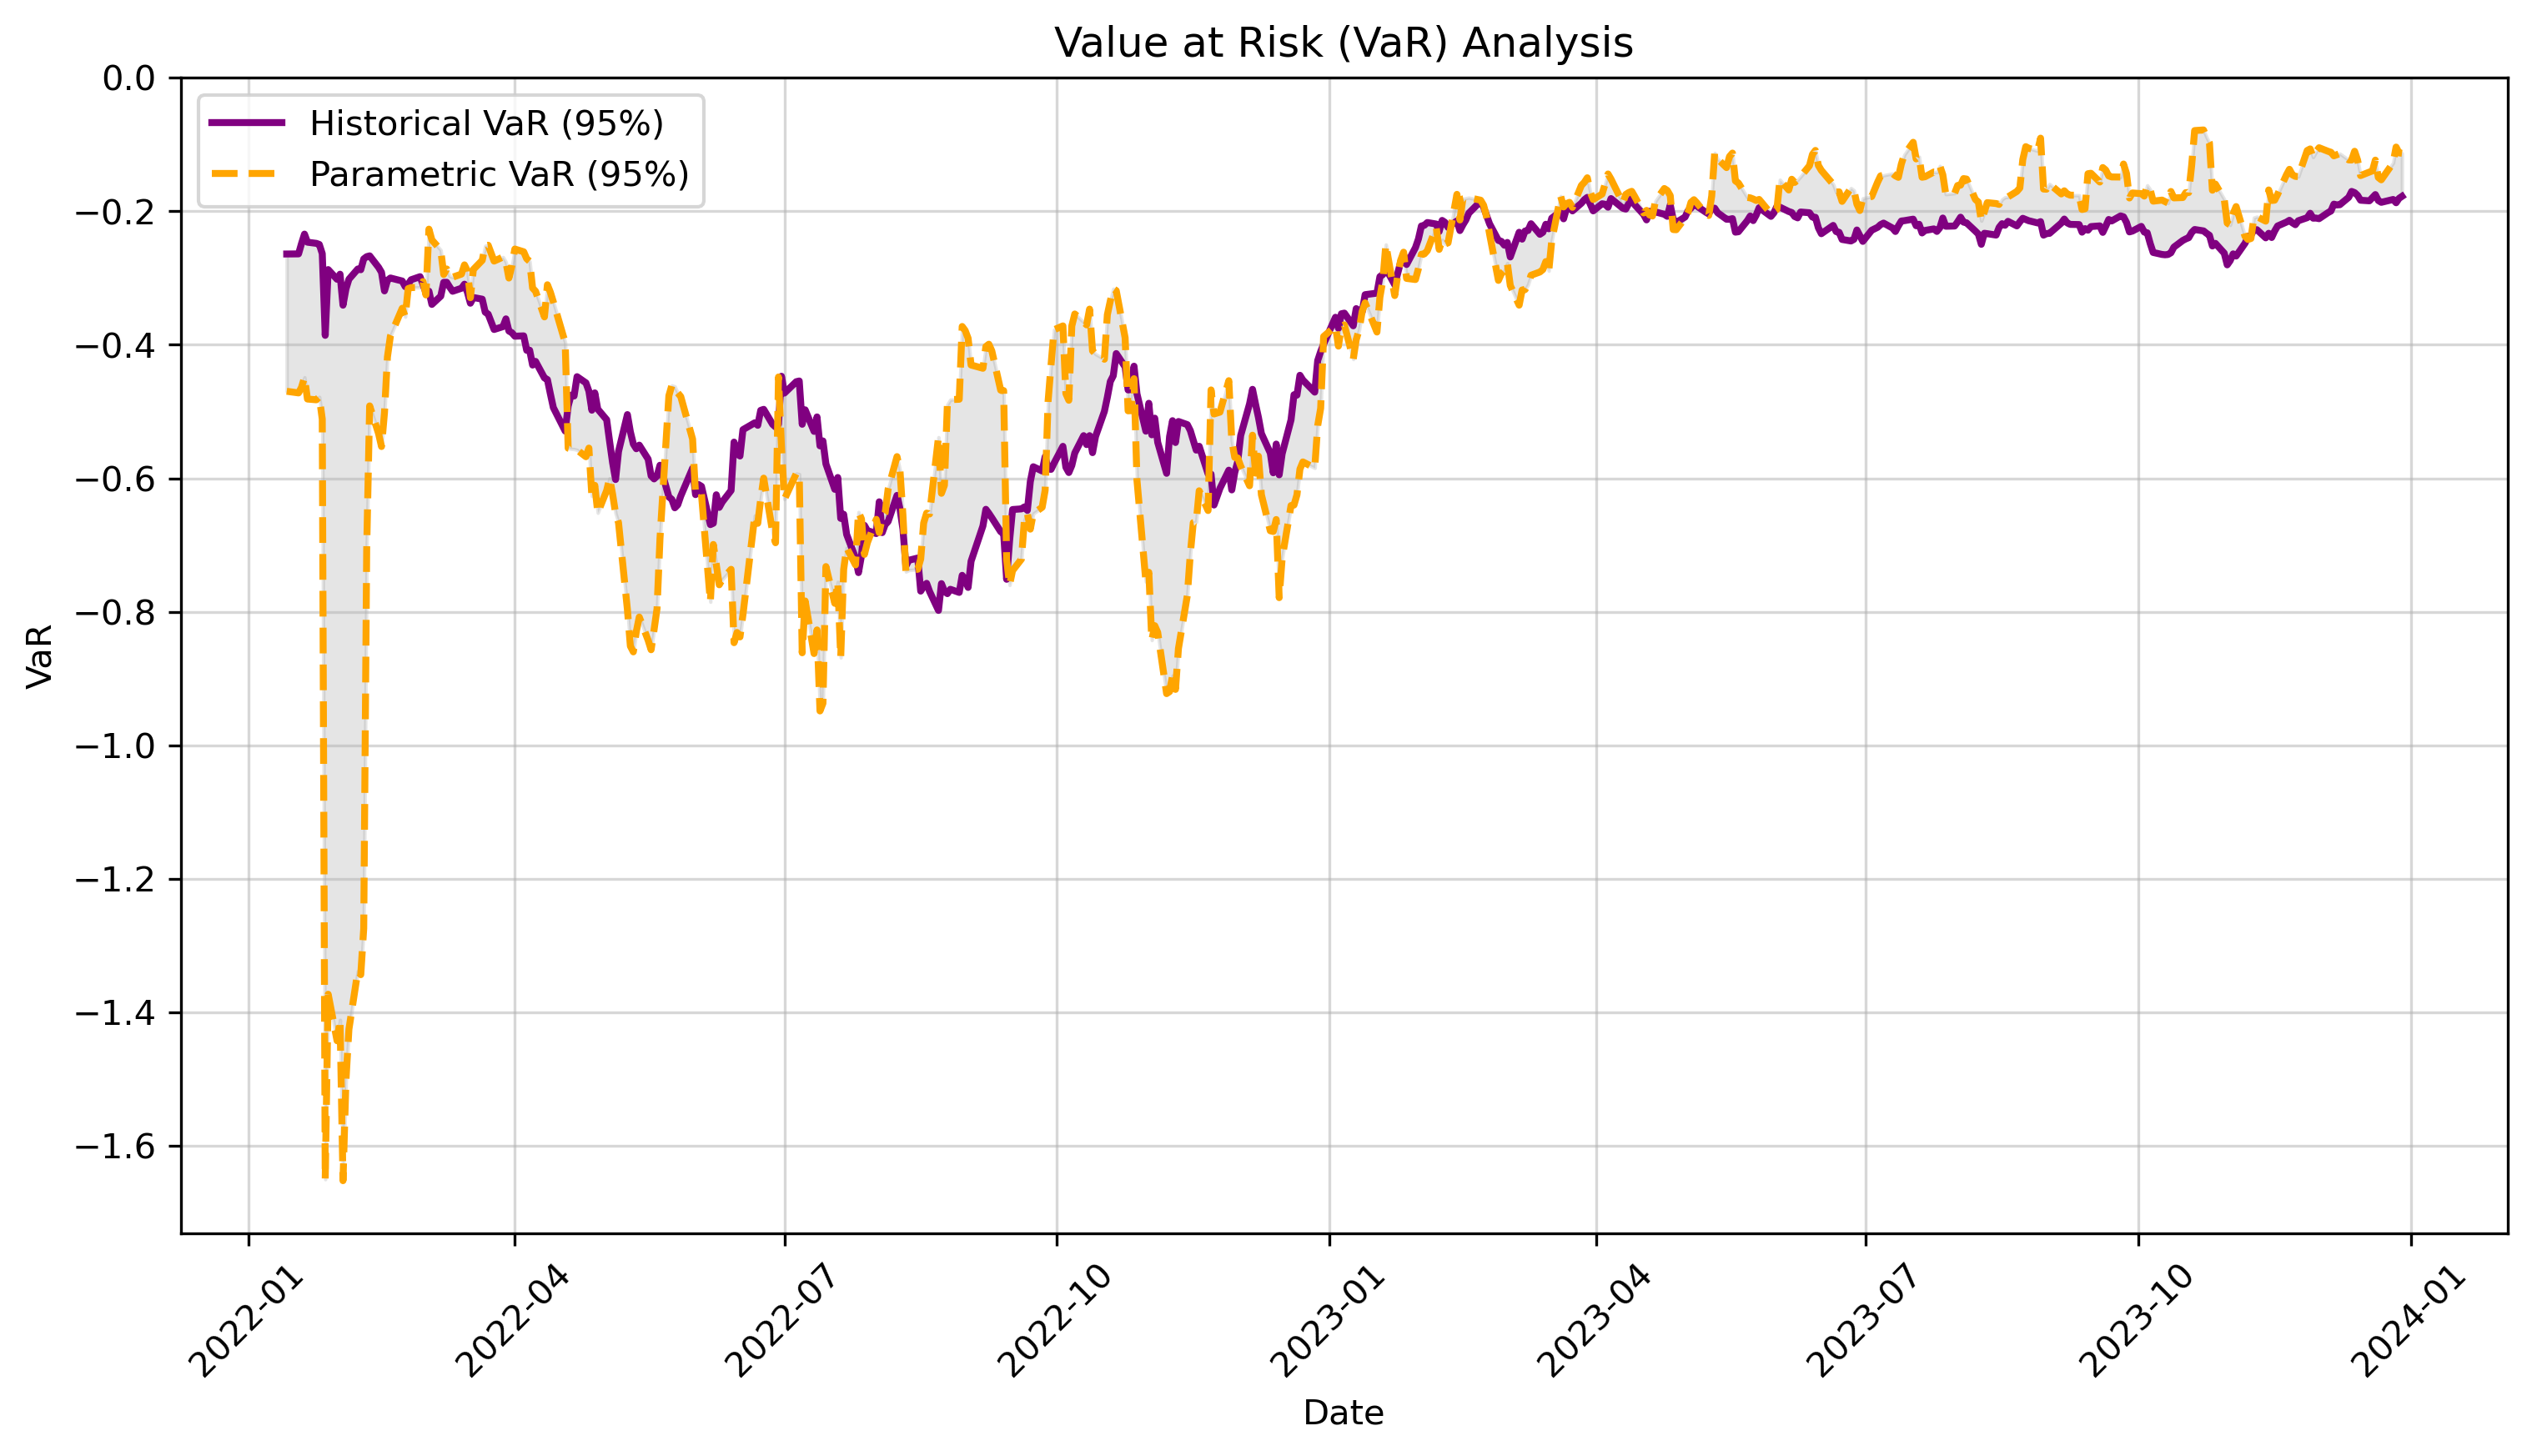
\includegraphics[width=0.85\textwidth]{value_at_risk_analysis.png}
    \caption{Value at Risk (VaR) Analysis: Comparing Historical VaR and Parametric VaR at a 95\% confidence level.}
    \label{fig:var_analysis}
\end{figure}
\FloatBarrier


% Inside the "Results and Analysis" section:
\vspace{1em}
\subsection{Feature Importance Analysis}
To understand which factors most influence margin requirements, we analyzed feature importance from the trained Random Forest model:
\vspace{2.5em}
\FloatBarrier % Ensures figures don't float to unexpected places
\begin{figure}[H]
    \centering
    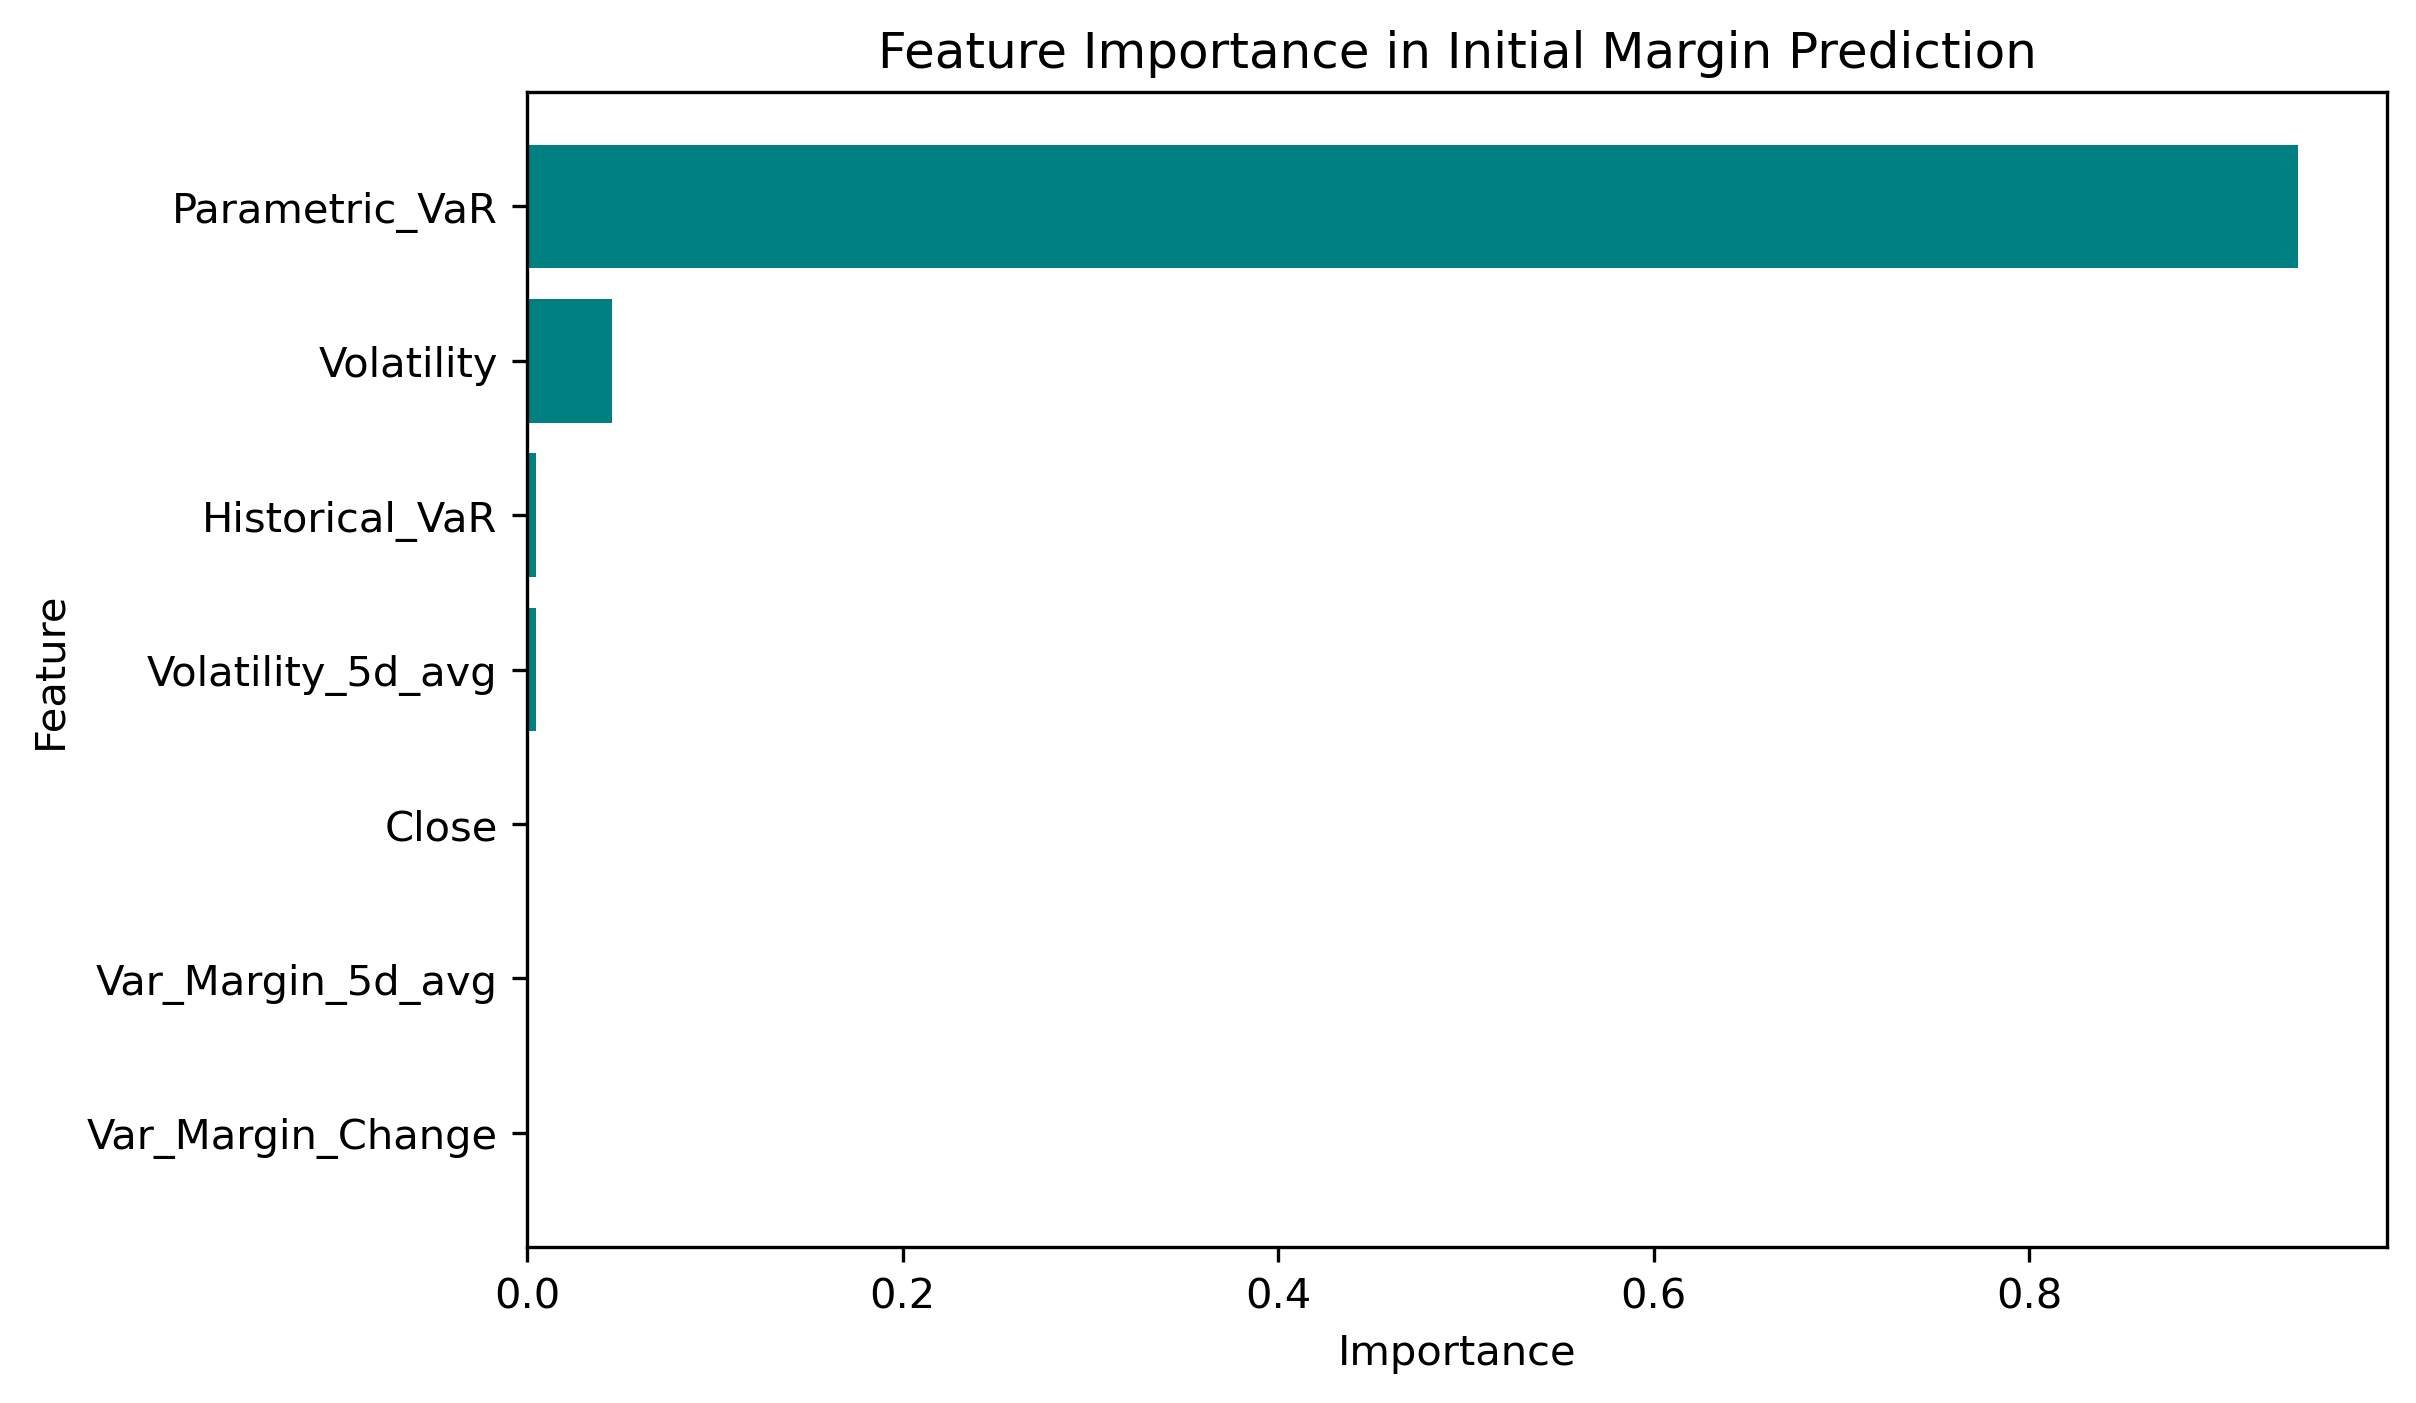
\includegraphics[width=0.85\textwidth]{feature_importance.png}
    \caption{Feature Importance in Initial Margin Prediction: Identifying key risk factors in margin estimation.}
    \label{fig:feature_importance}
\end{figure}


\begin{table}[h]
    \centering
    \begin{tabular}{lc}
    \toprule
    \textbf{Feature} & \textbf{Importance} \\
    \midrule
    Parametric VaR & 0.943214 \\
    Volatility & 0.045167 \\
    Historical VaR & 0.005312 \\
    Volatility 5d Avg & 0.004095 \\
    Var Margin 5d Avg & 0.002749 \\
    Var Margin Change & 0.002463 \\
    \bottomrule
    \end{tabular}
    \caption{Feature Importance in Initial Margin Prediction}
    \label{tab:feature_importance}
\end{table}

\FloatBarrier % Ensures the following content is properly placed

The results indicate that \textbf{Parametric VaR} is the most significant factor influencing initial margin, followed by \textbf{Volatility}. Historical VaR and short-term variations in margin have minor contributions.




\section{Limitations}
While this model offers a structured approach to margin calculation and risk analysis, it is not entirely accurate as it does not incorporate several broad market factors. Some key limitations include:
\begin{itemize}
    \item It does not implement advanced exchange-level margin methodologies such as SPAN.
    \item The model considers individual asset risk without integrating portfolio-level diversification effects.
    \item Real-time market conditions and news events, which significantly impact margin requirements, are not factored in.
    \item Extreme market shocks and stress testing scenarios are beyond the scope of this model.
\end{itemize}
Despite these limitations, this project serves as a fundamental framework that can be further developed into a more comprehensive risk management tool.




\section{Future Improvements}
To enhance the model, the following improvements can be made:
\begin{itemize}
    \item Implement SPAN-based margining methodologies.
    \item Incorporate real-time data and dynamic updates.
    \item Extend the model to support multi-asset portfolios.
    \item Introduce advanced risk metrics like Expected Shortfall (Conditional VaR).
\end{itemize}



\section{Conclusion}
This project successfully develops a computational tool for margin calculation and risk analysis in financial derivatives trading. By leveraging historical price data, statistical risk metrics, and machine learning techniques, the model provides a structured approach to estimating margin requirements. The findings highlight the critical role of volatility and Value at Risk (VaR) in determining initial margin, reinforcing their importance in risk management strategies used by financial institutions.
\vspace{1em}
The machine learning model, particularly the Random Forest Regressor, demonstrates strong predictive capability, achieving an R² score of 0.982 and a low Mean Squared Error (MSE), making it a reliable tool for estimating margin requirements. The feature importance analysis further validates the significance of Parametric VaR and market volatility in influencing margin levels. These insights contribute to better risk assessment practices, allowing traders, clearinghouses, and financial institutions to mitigate exposure to adverse market movements effectively.
\vspace{1em}
Despite the robustness of the model, there are certain limitations that need to be addressed. The current approach assumes a static risk factor and does not account for extreme market conditions such as financial crises, where volatility behaves unpredictably. Additionally, the model focuses on a single-asset margin calculation without considering portfolio diversification effects, which could significantly alter margin requirements in multi-asset trading environments.


\vspace{3em}

\section{References}
\begin{itemize}
    \item CME Group. ``SPAN Methodology.'' Available at: \url{https://www.cmegroup.com}
    \item Hull, J. ``Options, Futures, and Other Derivatives.'' Pearson Education.
    \item Yahoo Finance API Documentation. Available at: \url{https://www.yfinance.com}
\end{itemize}

\end{document}
